\documentclass[]{beamer}

% Use custom size to set poster's width and height.
\usepackage[scale=1.2, size=custom, width=120, height=100]{beamerposter} % use scale from 1.1 to 1.2
\usetheme{vegaposter} 


\addbibresource{refs.bib}
\usepackage{lipsum}

\title{To sell or not to sell: that is the question}
\author{Artemy Sazonov and Danil Legenkiy}
\supervisor{Anton Filatov, Vadim Mescheryakov}
\researchgroup{Currency Market Making}

\begin{document}
\nocite{*} % This is needed to make sure that all references are included in the bibliography

\begin{frame}[t]
    \begin{columns}[t] % The whole poster consists of three major columns, the second of which is split into two columns twice - the [t] option aligns each column's content to the top
     
    \begin{column}{\lrmargin}\end{column} % Empty spacer column
    
    \begin{column}{\onecolwid} % The first column
     
    %----------------------------------------------------------------------------------------
    %	INTRODUCTION
    %----------------------------------------------------------------------------------------
    
    \begin{block}{Introduction}
        Optimal trade execution is crucial in currency markets due to their high liquidity, continuous trading, and significant price impact. By studying and developing optimal execution approaches, researchers aim to provide practical tools and insights to enhance traders' performance, improve trade outcomes, and strengthen risk management capabilities in these fast-paced and global markets.
    \end{block}
    
    %----------------------------------------------------------------------------------------
    %	OBJECTIVES
    %----------------------------------------------------------------------------------------
        
    %------------------------------------------------
    \

    \begin{block}{Optimal execution problem statement}
        Liquidate the position by minimizing the functional of the price impact and the market risk. 
    \end{block}

    \

    \begin{alertblock}{Objectives}
    Here are the key steps of our research:
    \begin{itemize}
        \item Implement the MOEX L3 order book;

    	\item Calculate price-by-volume for the book;

    	\item Implement TWAP, AC and GLOBE;

    	\item Calculate the price impact metrics for the algorithms;

    	\item Compare the results.
    \end{itemize}
    
    \end{alertblock}


    \

    \begin{block}{Data collection and the OrderBook implementation}
        We obtained the L3 quote data for the four currency pairs from the MOEX:
        \begin{enumerate}
            \item USD/RUB; 
            \item EUR/RUB; 
            \item CHN/RUB;
            \item EUR/USD.
        \end{enumerate} 
        We implemented the order book in Rust using the B-tree as a base data structure. To our knowledge, 
        the ring buffer is considered to be the best practice in the industrial tasks for the order book storing, but we used 
        the B-tree due to the ease of the implementation.
    \end{block}



    
    %----------------------------------------------------------------------------------------
    
    \end{column} % End of the first column
    
    \begin{column}{\sepwid}\end{column} % Empty spacer column
    
    \begin{column}{\twocolwid} % Begin a column which is two columns wide (column 2)
    
    \begin{columns}[t,totalwidth=\twocolwid] % Split up the two columns wide column
    
    \begin{column}{\onecolwid}\vspace{-.6in} % The first column within column 2 (column 2.1)
    
    %----------------------------------------------------------------------------------------
    %	MATERIALS
    %----------------------------------------------------------------------------------------
    
    \begin{block}{Online ML}
        Online machine learning, also known as incremental or streaming machine learning, allows for the learning process to occur as new data becomes available. Unlike batch learning, where the algorithm is trained on a fixed dataset, online learning algorithms update their models iteratively, dynamically incorporating new observations into the learning process. This flexibility makes online machine learning well-suited for trade execution, where market conditions change rapidly and the ability to adapt quickly is crucial.
    \end{block}
    
    \

    %----------------------------------------------------------------------------------------
    
    \end{column} % End of column 2.1
        
    \begin{column}{\onecolwid}\vspace{-.6in} % The second column within column 2 (column 2.2)
    
    %----------------------------------------------------------------------------------------
    %	METHODS
    %----------------------------------------------------------------------------------------
    
    \begin{block}{Methods}
        We used \emph{Time-Weighted Average Price} (TWAP) as a baseline model.
        \begin{itemize}
            \item AC: introduced in \cite{Almgren2000}. We used the modification with linear impact functions when the closed-form solution for the optimal trading strategy is known.
            \item GLOBE: introduced in \cite{Akbarzadeh2018}. We used the custom-made modification which could be found by scanning the QR code. The original one has \emph{incredibly} many restrictions and complications.
        \end{itemize}
    \end{block}
    
    %----------------------------------------------------------------------------------------
    
    \end{column} % End of column 2.2
    
    \end{columns} % End of the split of column 2 - any content after this will now take up 2 columns width
    
    %----------------------------------------------------------------------------------------
    %	IMPORTANT RESULT
    %----------------------------------------------------------------------------------------
    
    \begin{alertblock}{Did you really believe it's going to be that simple?}
        \begin{enumerate}
            \item Both AC and GLOBE have \emph{significant} price impact \emph{restrictions}.
            \item The current order book implementation is \emph{static}.
            \item Because of 1 and 2, the proper backtest is restricted to \emph{mid-frequency execution only}.
            \item Because of 2 and 3, we need to write a \emph{virtual MOEX simulator}.
            \item Because of 1 and 3, we need to \emph{find a way to adapt} these algorithms to HFE.
        \end{enumerate} 
    \end{alertblock} 
    
    %----------------------------------------------------------------------------------------
    
    \begin{columns}[t,totalwidth=\twocolwid] % Split up the two columns wide column again
    
    \begin{column}{\onecolwid} % The first column within column 2 (column 2.1)
    
    %----------------------------------------------------------------------------------------
    %	MATHEMATICAL SECTION
    %----------------------------------------------------------------------------------------
    
    \begin{block}{A crash-course into HFT}
        We can divide all orders to 
        the two groups: \emph{market orders} (MO) and \emph{limit orders} (LO). 
        The LOs are \emph{passive}, the MOs are \emph{aggressive}.
        There is a thing called \emph{price impact} and it is the main reason why we should need to 
        optimize the trade execution. We have a trade-off between the 
        price impact and the market risk.
        The \emph{trading trajectory} is a process $(w_k)_{k = 0, \dots, L}$, where $w_k$ is a number of lots we 
        still posess at time $t_k$. Alternatively, we can define the \emph{trade list} $n_k = \Delta w_k$, $k = 1, \dots, L$ as a 
        number of lots we sell at time $t_k$.
        The \emph{trading strategy} is a rule for determining $n_k$ given the information avaliable at time $t_k$. Mathematically speaking,
        \begin{equation*}
            \hat n_k = \mathbb{E}^\nu\left[n_k\vert \mathcal{F}_{t_{k-1}}\right]. 
        \end{equation*} 

        \

        We can divide the strategies to \emph{static} (deterministic, all the parameters are known upon the start of the execution) and \emph{dynamic} (stochastic).
    

    \end{block}
   
    
    %----------------------------------------------------------------------------------------
    
    \end{column} % End of column 2.1
    
    \begin{column}{\onecolwid} % The second column within column 2 (column 2.2)
    
    %----------------------------------------------------------------------------------------
    %	RESULTS
    %----------------------------------------------------------------------------------------
    
    \begin{block}{Results}
    \vspace*{-1.5cm}
    \begin{figure}
        \hspace*{-1.5cm}
        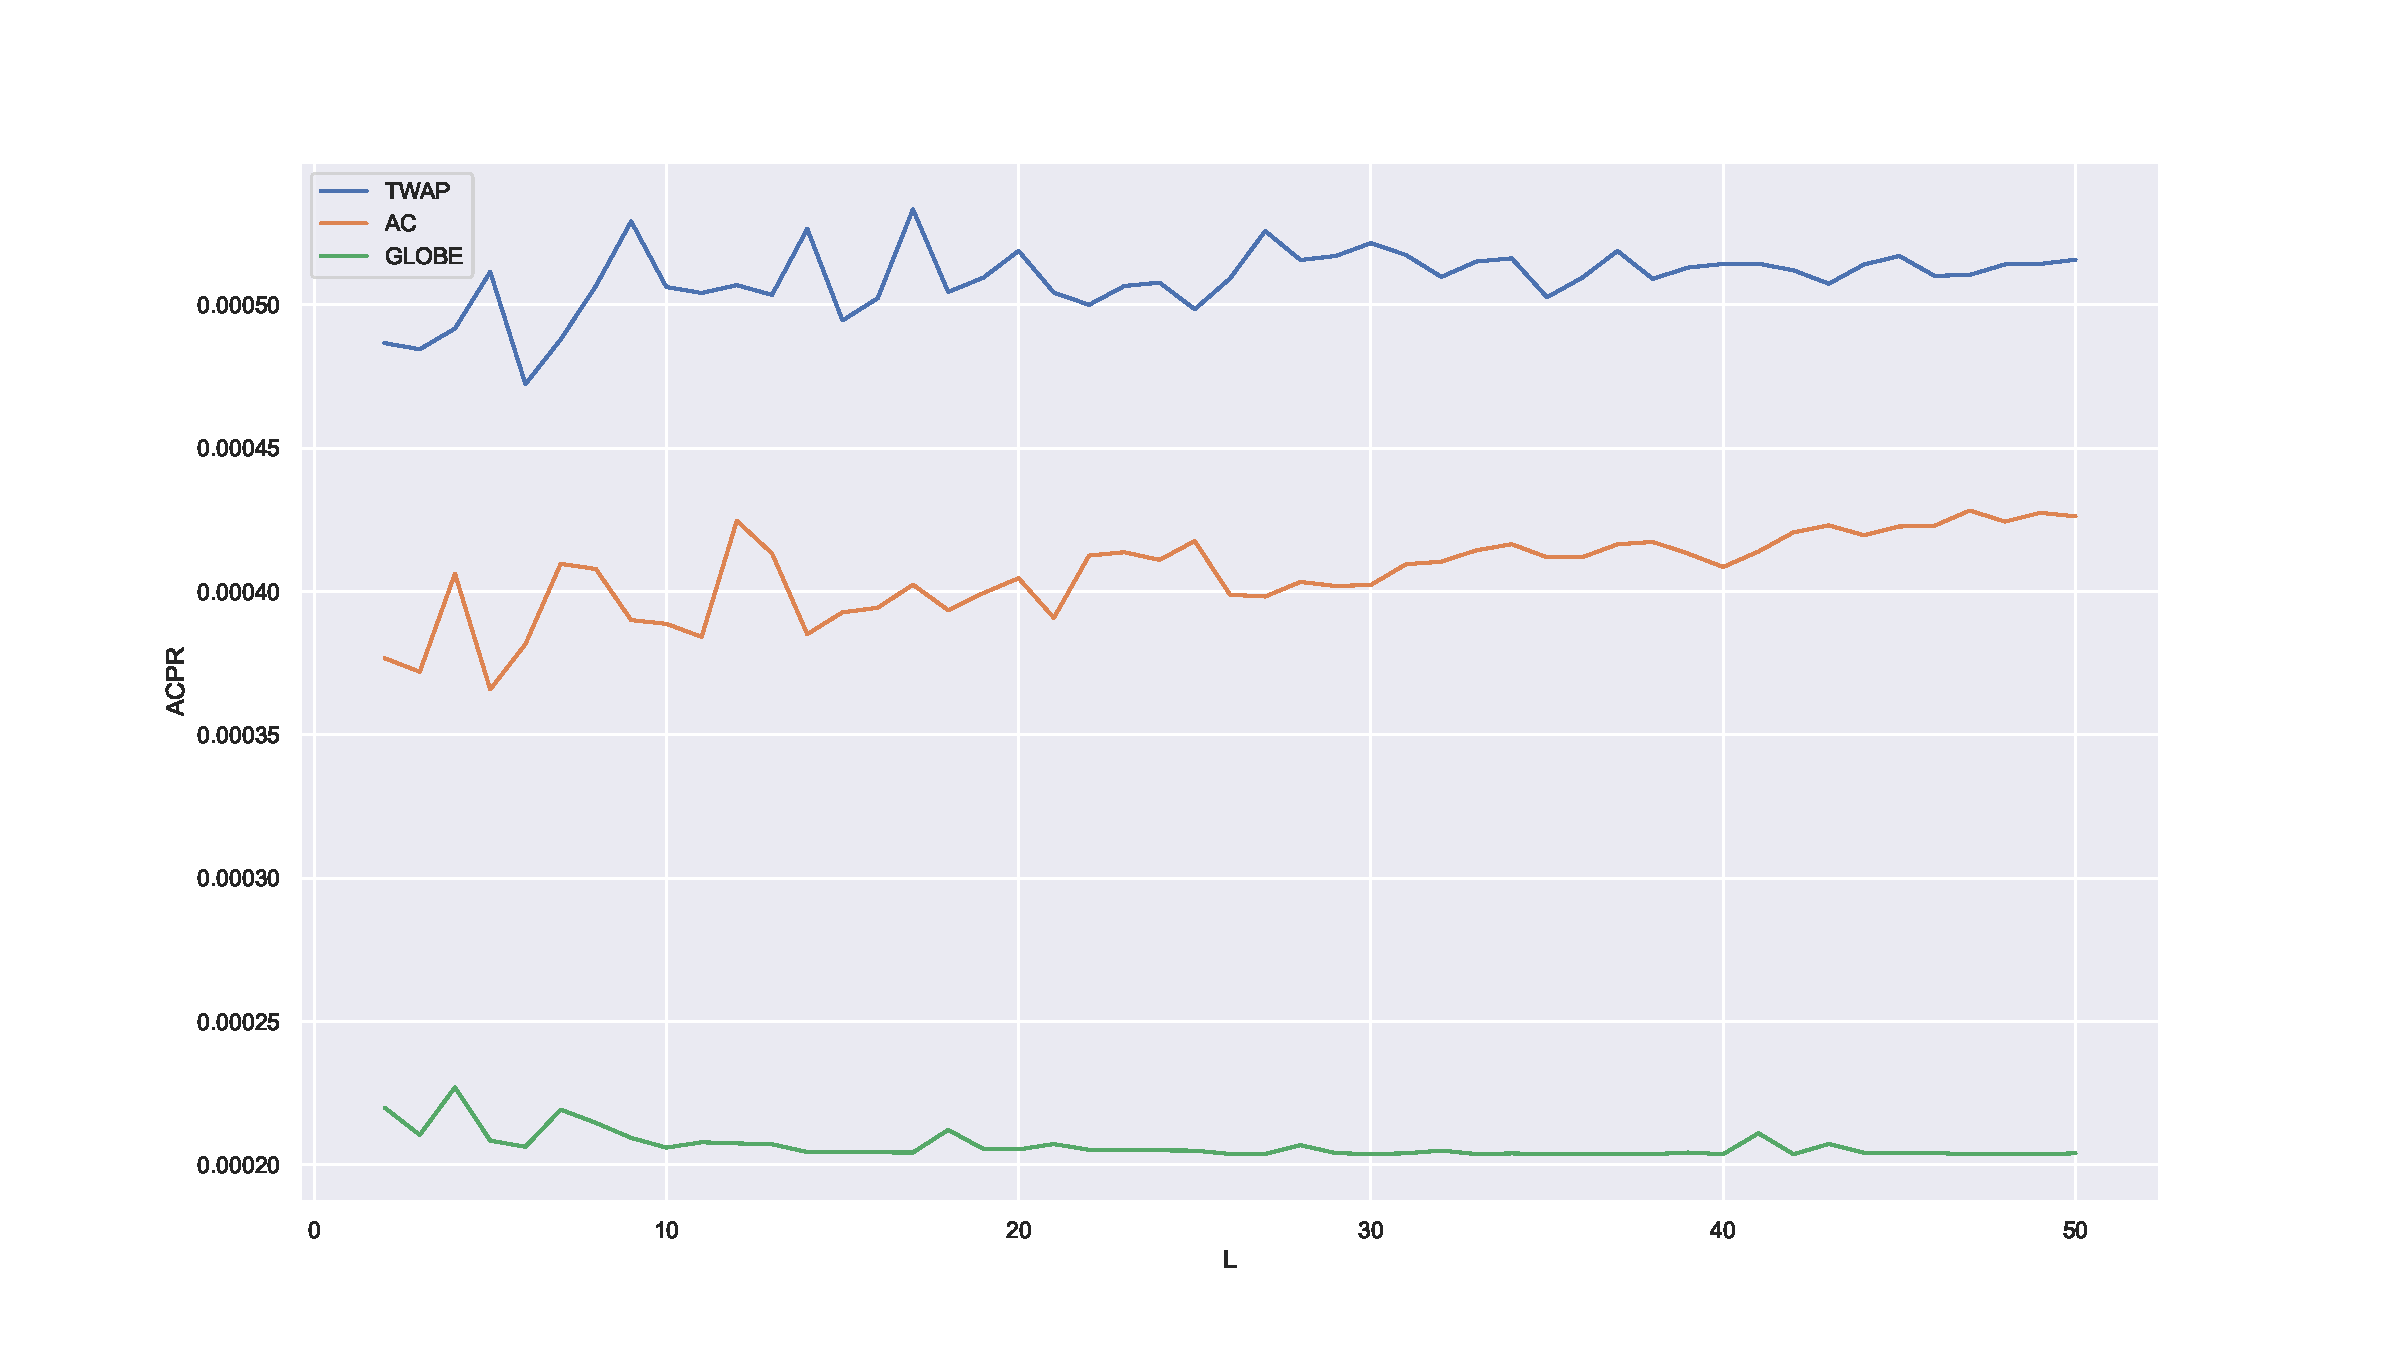
\includegraphics[width=1.1\linewidth]{figures/res1.pdf}
    \end{figure}
    \vspace*{-2.5cm}
    \begin{figure}
        \hspace*{-1.5cm}
        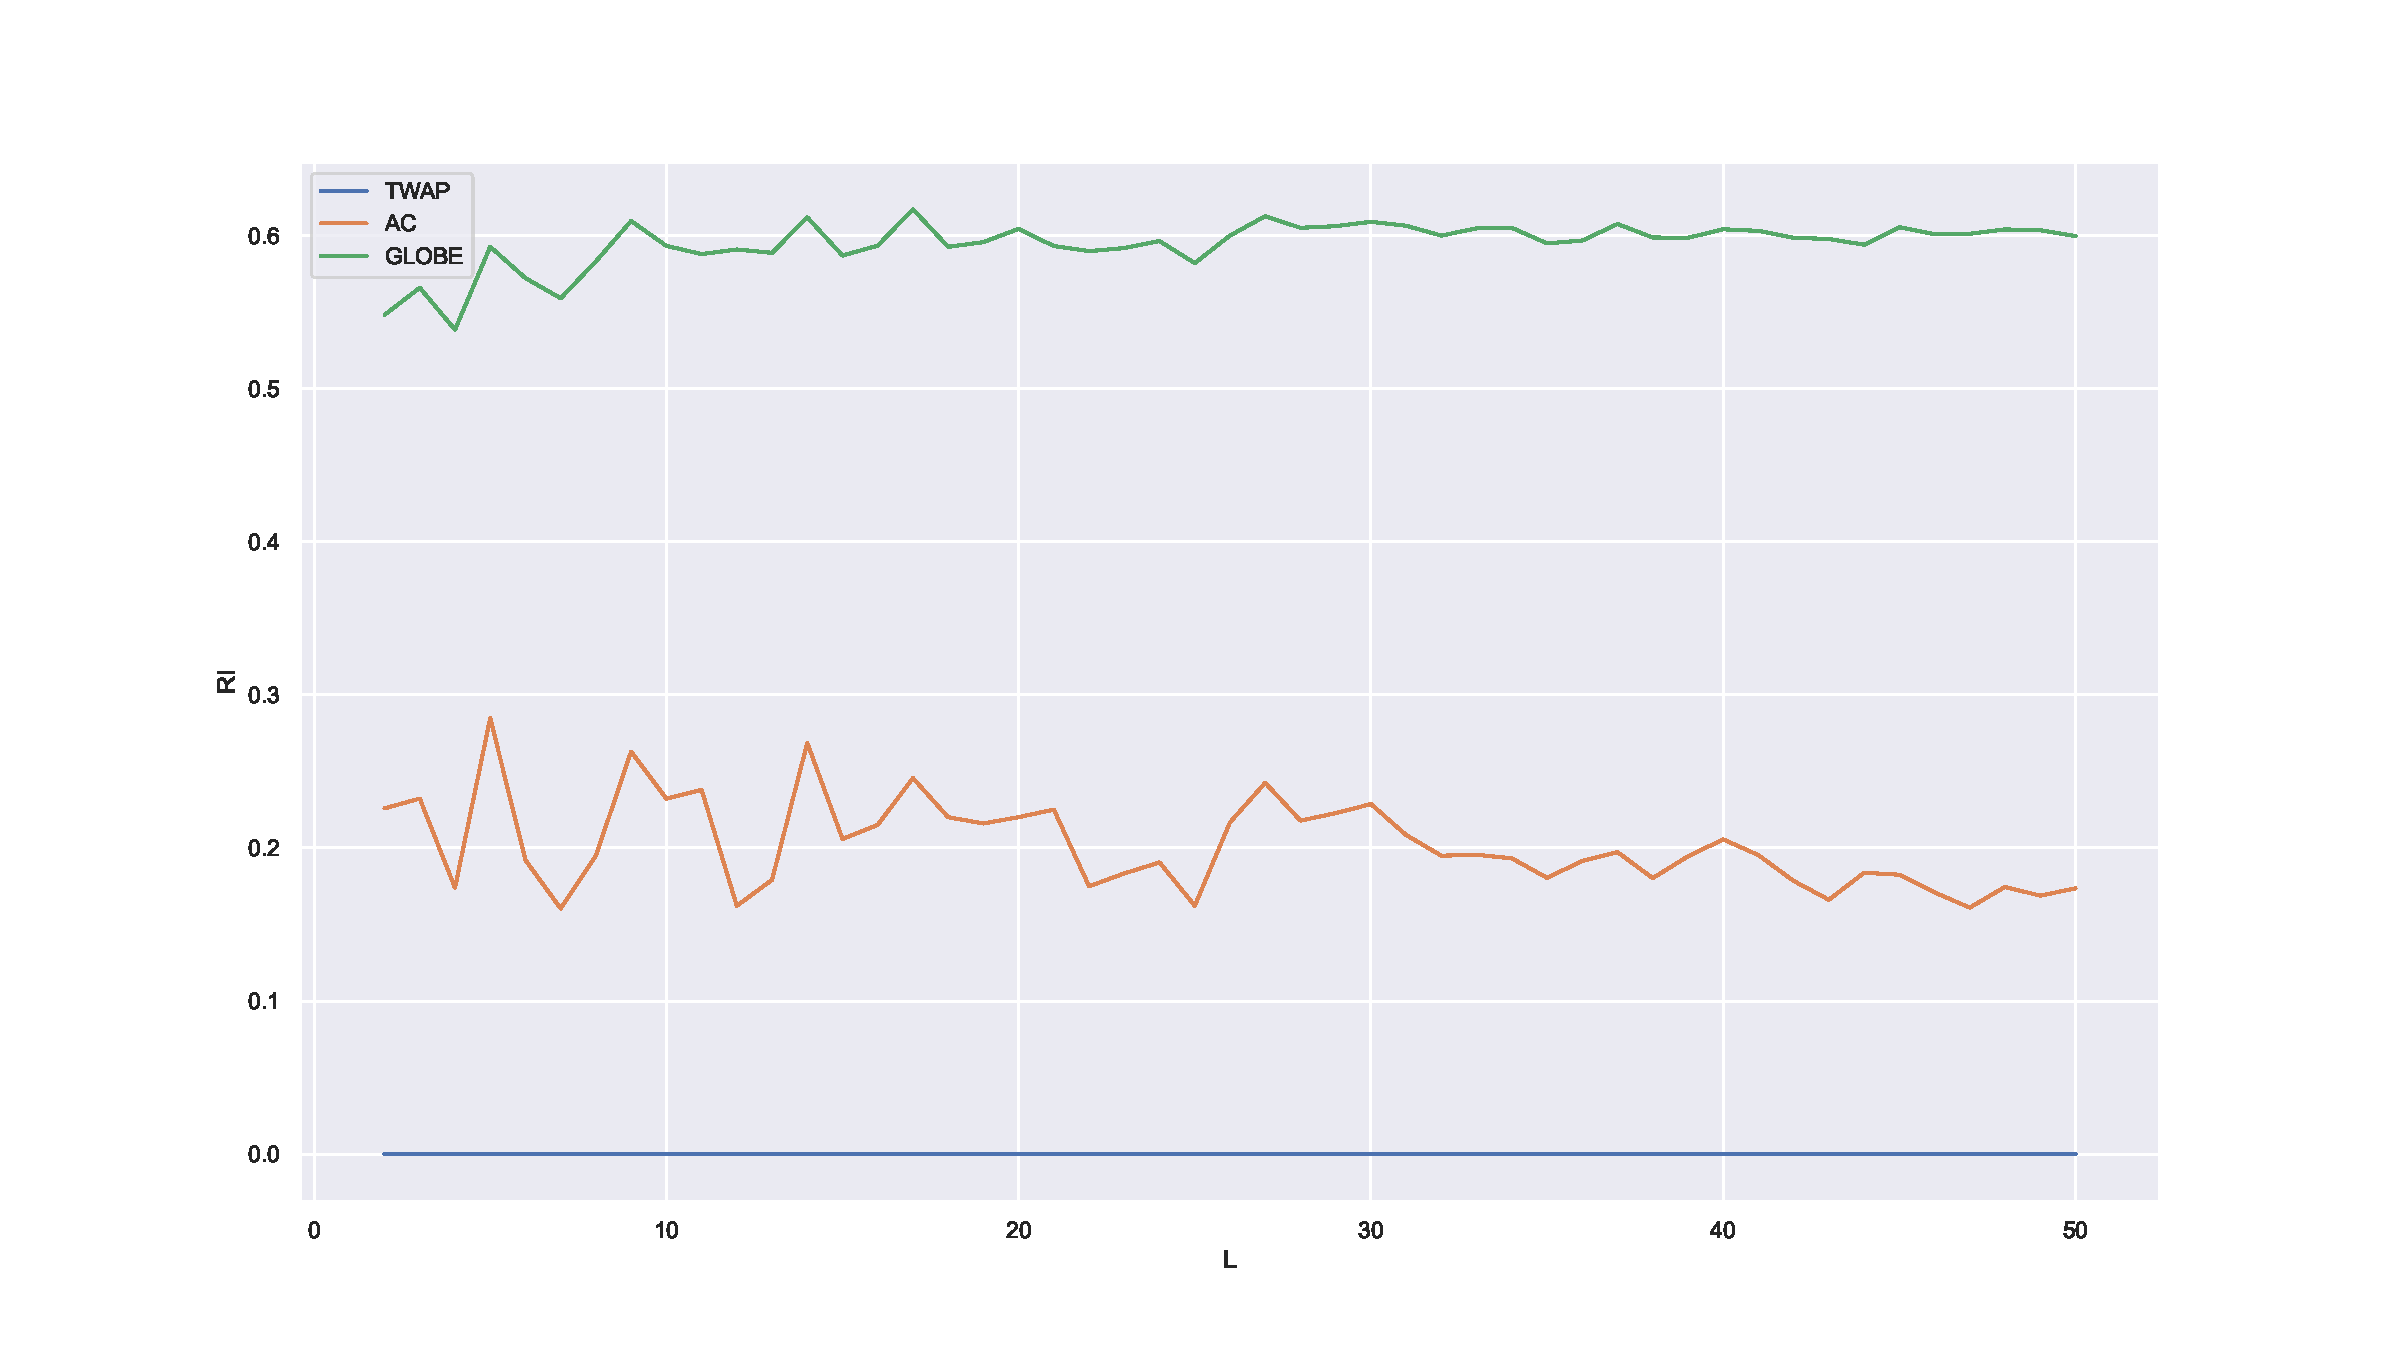
\includegraphics[width=1.1\linewidth]{figures/res2.pdf}
        \caption{ACPR and RI with TWAP as a baseline}
    \end{figure}
    
    \end{block}
    
    %----------------------------------------------------------------------------------------
    
    \end{column} % End of column 2.2
    
    \end{columns} % End of the split of column 2
    
    \end{column} % End of the second column
    
    \begin{column}{\sepwid}\end{column} % Empty spacer column
    
    \begin{column}{\onecolwid} % The third column
    
    %----------------------------------------------------------------------------------------
    %	CONCLUSION
    %----------------------------------------------------------------------------------------
    
    \begin{block}{Conclusion}
        During the semester we studied various books and articles about the market microstructure, high-frequency trading and market making.
        It is worth noticing that these topics are not usually covered by any standart courses or books.
        We implemented three trade execution algorithms:

        \begin{enumerate}
            \item Time-Weighted Average Price;
            \item Almgren-Chriss model with linear impact functions;
            \item Greedy exploration in Limit Order Book Execution.
        \end{enumerate}
        We found out that TWAP is the most versatile of them all, but is far from being the optimal one. 
        The AC model has the closed-form solution for the strategy only in case of the 
        linear price impact functions, and it's optimal strategy is deterministic.
        The underlying assumptions of the GLOBE algorithm do not allow us to use it for the high-frequency trading, and in 
        addition to that, the authors of this model stronly rely on the AC assumptions, which are not too realistic. 
    \end{block}
    
    \



    %----------------------------------------------------------------------------------------
    %	REFERENCES
    %----------------------------------------------------------------------------------------
    
    \begin{block}{References}
    
    \printbibliography
    
    \end{block}
    
    \end{column} % End of the third column
    
    \begin{column}{\lrmargin}\end{column} % Empty spacer column
    
    \end{columns} % End of all the columns in the poster
    \end{frame} % End of the enclosing frame
\end{document}